\chapter{Evaluation}\label{chp-eval}
\section{Overview}
To ensure that Labrador peforms correctly, I ran a series of statistical analyises on my evaluation crawls. These were designed to measure the effects of different partitioning schemes on the crawl and to compare these crawls to a run of Labrador in simple mode.

\section{Problems when evaluating crawlers}\label{sect-evalprobs}
It is particularly difficult to scientifically evaluate a web crawler. This eesentially stems from the fact that it is difficult to create a test environment. Although I ran many test crawls over different sizes of crawl domains, I restricted evaluations crawls to the websites of my department. This was because the amount of change of the website in any given time period is fairly small, meaning there is some hope that if two identical crawls were ran consecutively, they would produce the same results. I found that even in the departmental websites, a fluctuation of URLs fetched could vary between subsequent crawls in one day. This could be caused by additional pages being fetched, or by occasional transient errors created by the webserver under high load - typically this crawl runs at up to 55 URL/sec (averaged over a minute).\\
\ \\
Another external issue that affects the outcome of the crawl is the background network load and server load being experienced during the duration of the crawls. While a crawl may last a couple of hours, network usage may vary from hour to hour (e.g. higher usage during lunch time), and from day to day. This may adversly affect the crawl, but any effect is difficult to measure.

\section{Partitioning}\label{sect-evalpartitioning}
\subsection{Background}
As dicussed in Section \ref{sect-partitioning}, I implemented two modes for Labrador to operate in: Simple; and Partitioned mode. This set of evaluation was performed to compare the crawler over. Three crawls were operated, as described in Table \ref{tbl-partcrawls}.\\
\begin{table}
\begin{center}
\begin{tabular}{|l|l|l|}
\hline
\bf{Name} & \bf{Mode} & \bf{Partitioning} \\
\hline
Crawl 1 & Simple & N/A \\
\hline
Crawl 2 & Partitioned & MultiHostDirectory \\
\hline
Crawl 3 & Partitioned & MultiHostTopDirectory \\
\hline
\end{tabular}
\end{center}
\caption{Evaluation Crawls}\label{tbl-partcrawls}
\end{table}

Each crawl was seeded with only six URLs, the six departmental home pages. They are listed in Table \ref{tbl-smallseeds}.\\
\begin{table}
\begin{center}
\begin{tabular}{|l|}
\hline
\bf{URL} \\
\hline
http://www.dcs.gla.ac.uk/\# \\
\hline
http://www.brc.dcs.gla.ac.uk/\# \\
\hline
http://tlc.dcs.gla.ac.uk/\# \\
\hline
http://ir.dcs.gla.ac.uk/\# \\
\hline
http://grumps.dcs.gla.ac.uk/\# \\
\hline
http://faraday.dcs.gla.ac.uk/\# \\
\hline
\end{tabular}
\end{center}
\caption{Evaluation Crawl - Seed URLs}\label{tbl-smallseeds}
\end{table}


\subsection{Crawl time}
Figure \ref{fig-crawlgraphs} shows URLs fetched by the crawls described in Section \ref{tbl-partcrawls}. It clearly shows that Crawl 3, using the MultiHostTopDirectory scheme was the fastest. The Simple mode crawler was the slowest.\\
\ \\
I expected the Simple mode crawler to be the slowest, as each crawler (8 in this case) must communicate with the dispatcher between every URL. This creates a bottleneck at the dispatcher. MultiHostTopDirectory performed best as its partitions are larger, meaning less inter-partition linkage. When a crawler discovered a link outwith its own partition it has to send it back to the dispatcher. For instance, each lecturer has their home page at http://www.dcs.gla.ac.uk/$\sim$username/. I theorise that most of the links in each lecturers home page create to their own material, which when using MultiHostTopDirectory is in the same partition. However under MultiHostDirectory, sub-directories are a different partition, which means that those links must be sent back to the dispatcher.\\
\ \\
The astute reader may notice that the three crawls did not fetch the same number of URLs, for the reasons described in Section \ref{sect-evalprobs}. Furthermore, all three crawls suffered a drop in rate at approximately 50,000 URLs (although less prononuced in Crawl 3). I theorise that crawls of the departmental website become involved in the Bibliography database around that point. As each bibliography page requires a database fetch, the time taken to fetch the rate is higher, which ultimately affects the fetch rate. Further investigation would be required to validate this theory.
\begin{figure}[h]
  \centerline{
    \epsfig{file=./images/finished.ps, scale=0.60, angle=-90}
   }
\caption{Comparision of Crawls 1, 2 \& 3}\label{fig-crawlgraphs}
\end{figure}
\subsection{Dispatcher CPU Usage and Network I/O}
Table \ref{tbl-evalresources} shows the resources consumed by the dispatcher during the three crawls. It can clearly be seen that Network Output of the dispatcher is greatly reduced by using a partitioned crawler and Crawl 3 is the best case in all measurements. Crawl 2 appears to be worse than Crawl 1 in the processing time and Network Input fields, yet is only slightly worse than Crawl 3 in Network output. Had more time been available, I might have run multiple crawls and averaged results to validate this trend.
\begin{table}
\begin{center}
\begin{tabular}{|l|l|l|l|}
\hline
\bf{Crawl} & \bf{Dispatcher User Time} & \bf{Network In} & \bf{Network Out} \\
\hline
Crawl 1 & 82.94 Secs & 23.66MB & 70.29MB \\
\hline
Crawl 2 & 102.1 Secs & 37.82MB & 5.97MB \\
\hline
Crawl 3 & 60.23 Secs & 13.79MB & 2.77MB \\
\hline
\end{tabular}
\caption{Resource Usage for Crawls 1, 2 \& 3}\label{tbl-evalresources}
\end{center}
\end{table}

\section{Content Filtering}
Table \ref{tbl-evalcontentfilters} shows how effective the two ContentFilters are at detecting duplicate and binary content. Given that all exact duplicates in a website seem to be under 10\%, it would be interesting to determine if duplicate and binary files would be a good indicator of the administration quality of a website. For instance, a good webmaster will not simply copy content, but will instead add a redirect and move the content. Similarly, the binary filter only picks up files that have an incorrect content type sent by the server, which is a configuration issue with the server.
\begin{table}
\begin{center}
\begin{tabular}{|l|l|l|l|}
\hline
\bf{Crawl} & \bf{Duplicates Found} & \bf{Binary Files Found} & \bf{URLs Fetched} \\
\hline
dcs.gla.ac.uk & 3356 (5.6\%) & 179 & 59702 \\
\hline
gcal.ac.uk & 247 (2.9\%) & 0 & 8601 \\
\hline
paisley.ac.uk & 349 (8.6\%) & 1 & 4021 \\
\hline
\end{tabular}
\caption{Content Filter usage in Test Crawls}\label{tbl-evalcontentfilters}
\end{center}
\end{table}


\section{Discovery}
\subsection{Background}
I was interested to see how much faster a crawl of the departmental websites would be if the crawler was seeded with all the URLs of the site. 
\subsection{Results}
The results of this crawl (Crawl 4 in Figure \ref{fig-crawl4}) were slightly dissapointing. As the crawl is seeded with all known URLs in the website, the discovery period is nil and the crawler should fetch at its highest possible rate. This appears to be happenning until about 1000 seconds have passed. At this time, many crawlers appeared to timeout and disconnect, leaving only one crawler to finish the rest of the work. This can be seen in Figure \ref{fig-crawl4_connections}, which shows the number of crawlers connected to the disptacher over the duration of the crawl (one connection is used by the monitoring software). Crawlers only disconnect when they have been allocated no work for 500 seconds. I theorise that the seeding of URLs has caused one crawler to grab most of the partitions, leaving it to perform all the work. Hence, this shows more work should be performed in acheiving a fair allocation of partitions between the available crawlers.\\
\\ \
Also of note in Figure \ref{fig-crawl4} is the changes in fetch rate experienced by the crawler. I theorise here that the ordering of the rootset has placed many bibliography database URLs closer together, meaning that the database server serving those pages has become slow due to high usage. These occur at times 2500-4000 and 5000-6000. The department perform insufficient monitoring on their database servers to check the loading at the times of interest. However, subsequent crawls found maximum CPU usage on the database server when the crawl was requesting URLs from the bibliography and contacts databases.
\begin{figure}[h]
  \centerline{
    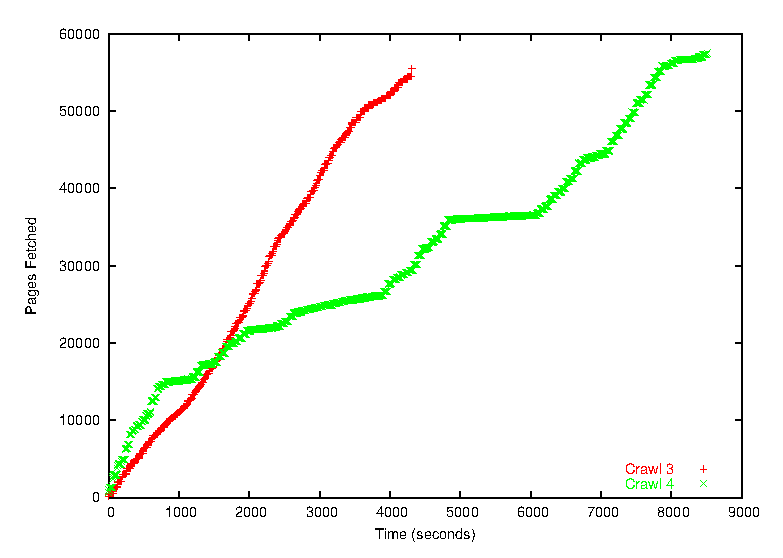
\epsfig{file=./images/crawl4.eps, scale=1.0}
   }
\label{fig-crawl4}
\caption{Crawl 4 (Green) - Seeded with all URLs}
\end{figure}

\begin{figure}[h]
  \centerline{
    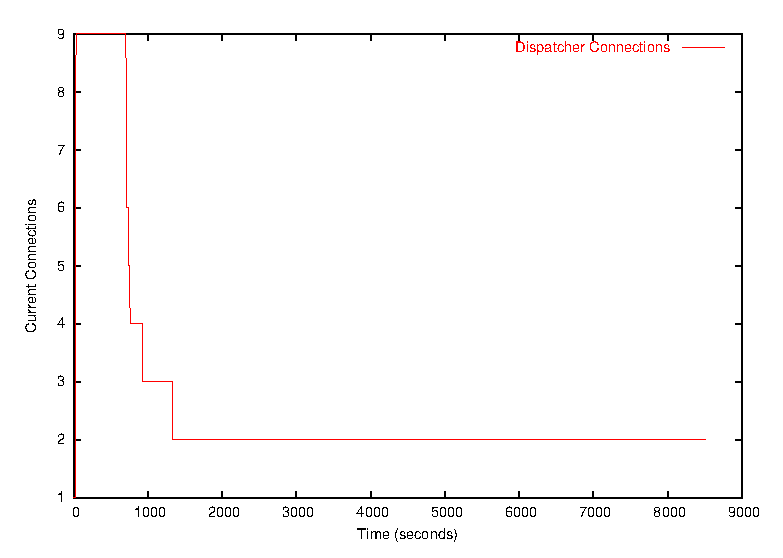
\epsfig{file=./images/crawl4-connections.eps, scale=1.0}
   }
\label{fig-crawl4_connections}
\caption{Crawl 4 - Number of Dispatcher Network Connections}
\end{figure}

\section{PL2 Changes in relation to crawl size}\label{sect-evalpl2}
In Section \ref{sect-terriermatching}, I described the PL2 matching model used by Terrier. He and Ounis describe\cite{ref13} a way of optimising DFR models, such as PL2. This involved tuning the $c$ parameter to acheieve normalisation of term weight to average document length. This is because, in IR, it is current practice to normalise term weight in respect to the length of the document. The c parameter is best normalised for different query sizes.\\
My results are shown in Table \ref{tbl-pl2values} and Figure \ref{fig-pl2}.
\begin{figure}[h]
  \centerline{
    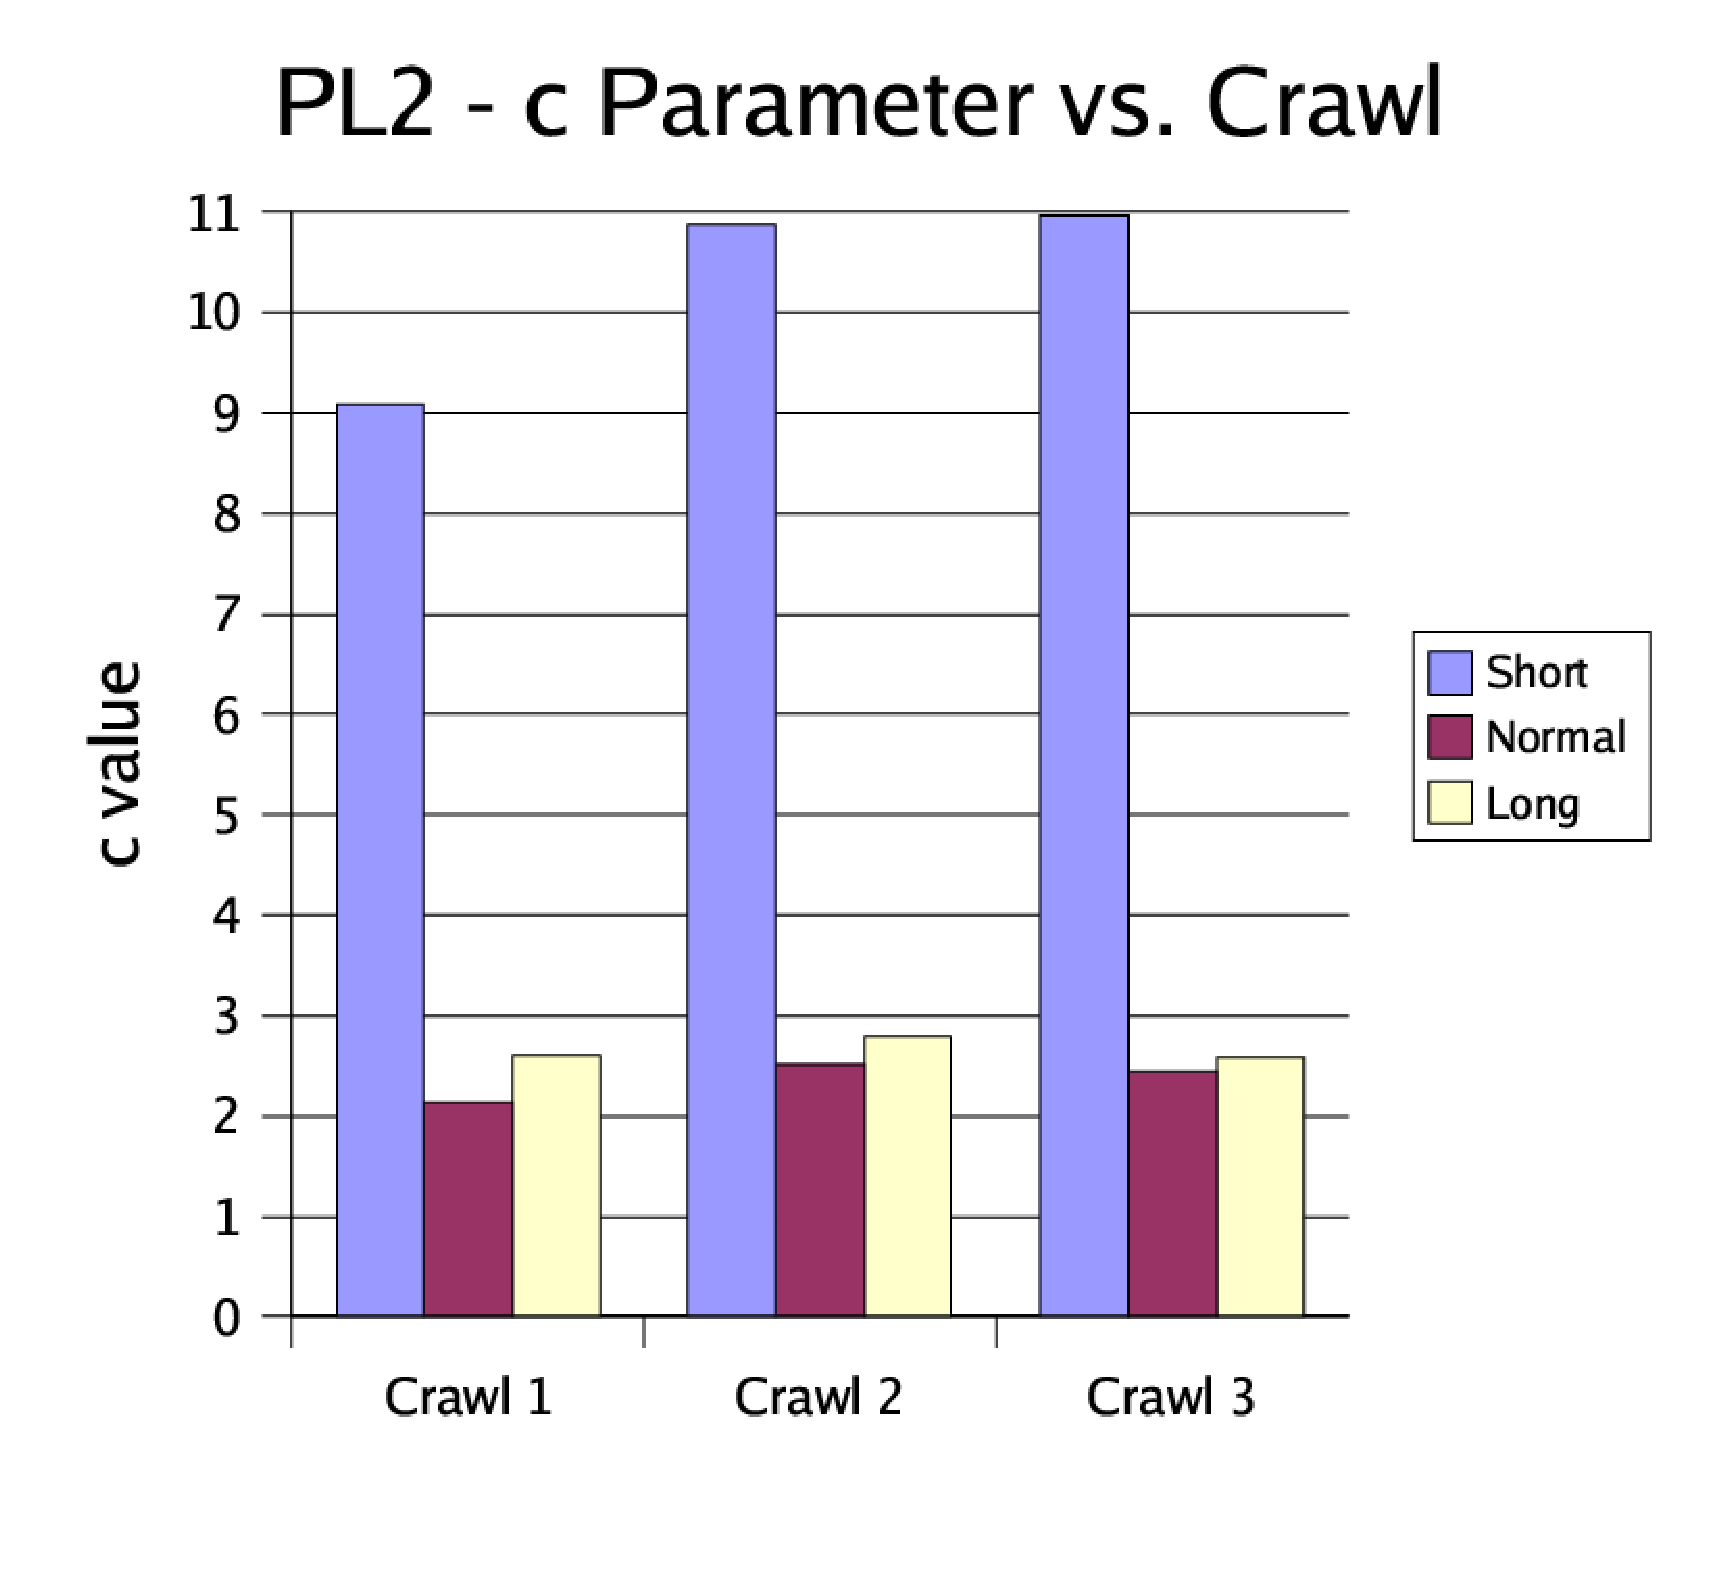
\epsfig{file=./images/graph_pl2c.eps, scale = 0.4}
   }
\label{fig-pl2}
\caption{Affect of increasing crawl size on PL2's $c$ parameter}
\end{figure}
\begin{center}
\begin{table}
\begin{tabular}{|l|l|l|l|}
\hline
\bf{Crawl} & \bf{Query length 1 to 5 words} & \bf{Query length 5 to 12 words} & \bf{Query length more than 12 words} \\
\hline
Crawl 1 & 9.09 & 2.14 & 2.60 \\
\hline
Crawl 2 & 10.88 & 2.51 & 2.79 \\
\hline
Crawl 3 & 10.96 & 2.45 & 2.58 \\
\hline
\end{tabular}
\label{tbl-pl2values}\caption{$c$ Values for different crawls}
\end{table}
\end{center}
This evaluation was performed using three crawls: 1. All externally accessable websites from the Department of Computing Science, Glasgow University; 2. All externally accessable websites of Glasgow University; 3. All externally websites of the Glasgow, Strathclyde, Glasgow Caledonian and Paisley Universities.

\section{Summary}
This evaluation showed the effectiveness of the partitioned mode of the Labrador crawler and of the content filters installed to identify unwanted content during crawls. Test crawls not discussed here show that Labrador can scale to fetching up to millions of pages. I have shown that Discovery period for recrawls could be minimised by seeding the crawl with more URLs, but that care needs to be made in how the seed URLs are partitioned between crawlers. Additionally, the properties of the $c$ parameter of the PL2 DFR matching model over collections has been investigated.
